\documentclass{article}

\usepackage[letterpaper, top=2cm, bottom=2cm, left=2cm, right=2cm]{geometry}
\usepackage[english]{babel}
\usepackage{multicol}
\usepackage{enumitem}
\usepackage[fontsize=10]{scrextend}
\usepackage{romannum}
\usepackage{graphicx}
\AtBeginDocument{\pagenumbering{arabic}} %coz romannum-package changes page nunber

\begin{document}
\setcounter{page}{102}
\begin{multicols}{2}


\begin{enumerate}[noitemsep]
\setcounter{enumi}{1}
\item[] significantly reduces its accuracy [11]. It is proposed
to exclude anomalous predictions by using a truncated arithmetic mean [12] [13].
\item 
Methods based on minimizing the final forecast
error by the least squares method [14].

\item 
Methods based on minimizing the variance of
the combined forecast error (works by Bates and
Granger [6], Ershov [15], Baltrushevich [16]).

\item Methods based on retrospective forecasts. This
group includes the AFTER method [17]. The
weights of the private forecasts are calculated based
on their own past values, conditional variance, and
the past values of the private forecasts. The weights
are updated after each new observation.
The following disadvantages of the AFTER method
were noted in [8]:

\begin{itemize}[noitemsep]
    \item difficult applicability in practice;
    \item strong dependence of the weights on the first set
value. 
\end{itemize}
This group includes the following methods:
\begin{itemize}[noitemsep]
    \item ARM, developed by Yang [18];
    \item the Bunn method [19], which assumes finding
the distribution function for the weight coefficient
through the beta distribution;
    \item an adaptive method based on exponential smoothing [2], [20].
\end{itemize}

\item Methods based on factor analysis. These methods
were proposed by Frenkel [21] and Gorelik and
Frenkel [5]. The idea of using factor analysis is
based on the fact that particular forecast results
using a separate forecasting method are an external
expression of some really existing but immeasurable
forecast value, which is taken as a combined forecast
[8].
\item The method of Gupta and Wilton, based on finding
the optimal weights of the coefficients of particular
predictions using a matrix of pairwise preferences,
has been placed in a separate group [22].
\item Methods based on quadratic programming. The
paper [23] describes a method for calculating the
weights of particular predictions by minimizing the
retrospective relative errors of particular predictions
using quadratic programming methods.



\end{enumerate}
\par The main advantage of the method is efficiency and
ease of implementation. The main disadvantage is the
obligatory preliminary selection of particular forecasting
methods in order to comply with the requirement of error
independence [8]. 
\par Most of the methods for combining forecasts are based
on the assumptions about the independence of the abso-
lute forecast errors and their distribution in accordance
with the normal law with zero mathematical expectation
and unknown variance. However, these assumptions are
often not met [3], and therefore, methods based on fuzzy 
logic and stable statistical estimates are currently being
actively developed, for example:


\columnbreak

\begin{enumerate}[noitemsep]
    \item method of combining forecasts by Kovalev [24]
based on a system of fuzzy rules;
    \item he Davydov union method [25], based on the use
of a robust M-estimate;
    \item Methods for combining particular forecasts by
Vasiliev [26] based on the robust Huber estimate
of the truncated mean type and on the basis of the
Hodges-Lehmann R-estimate.
\end{enumerate}

Thus, despite a significant number of publications
on the topics of forecasting methods for time series
and methods for aggregating individual forecasts, the
question of choosing the most appropriate aggregating
method and its constituent forecasting models for the
predicted time series remains. 
\begin{enumerate}[wide, labelindent=0pt]
\item[] \Romannum{2}. Developed algorithm for calculating the 
\centerline{aggregated
forecast of time series}
\end{enumerate}

\par Figure 1 shows a schematic description of the devel-
oped algorithm for calculating the aggregated forecast of
time series.

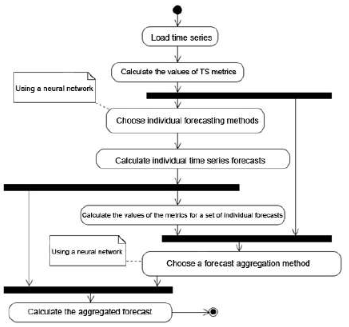
\includegraphics{pivo3}
\small Figure 1. Algorithm for calculating the aggregated forecast of time
series
\par In this paper, 2 methods of setting the forecast weights
are considered:
\begin{itemize}[noitemsep]
    \item [--] the first method is based on the values of the
prediction error on the control part of the time
series;
    \item [--] the second method is based on the error values
assumed by the neural network for choosing a
prediction method.
\end{itemize}
The structure of the neural network for choosing the
aggregating method is close to the structure of the neural
network for choosing individual prediction methods, but
it includes more input neurons corresponding to the
metrics. Neurons corresponding to individual prediction

\end{multicols}
\end{document}
